% begin module trig-substitutions-ex3-version-2
\begin{frame}
\begin{example}[$\ds \int \frac{1}{x^2 \sqrt{x^2+4}}\diff x$] %[Example 3, p. 505]
\begin{columns}[c]
\column{.6\textwidth}
\begin{itemize}
\item<2-> $ \sqrt{x^2+a^2} $: $ x=a\tan\theta $
\item<3->  Let $x = \uncover<4->{2\tan \theta}$ \uncover<4->{,   $-\pi /2 \leq \theta \leq \pi / 2$.}
\item<5->  Then $ \tan\theta=\frac{x}{2},  $ and $\diff x = \uncover<6->{2\sec^2 \theta\diff \theta}$ \uncover<7->{. \\ Build a triangle.}
\end{itemize}
\column{.4\textwidth}
\begin{center}
\uncover<8->{
\psset{xunit=1.5cm, yunit=1.5cm}
\begin{pspicture}(-0.15,-0.3)(2.3,1.2)
\psframe*[linecolor=white](-0.1,-0.3)(2.3,1.2)
\psline(0,0)(2, 0)(2,1)(0,0)
\psline(1.9,0)(1.9, 0.1)(2,0.1)
\fcAngle{0}{0.463648}{0.4}{$\theta$}
\uncover<handout:0|9->{
\rput[l](2.1, 0.5){$x$}
\rput[t](1, -0.1){$2$}
}
\uncover<handout:0|10->{
\rput[br](1, 0.55){$\sqrt{x^2+4}$}
}
%bounding box for pdflatex compilation:
\psline[linecolor=red!1](-0.11, -0.3 )(-0.105, -0.3)
\psline[linecolor=red!1](2.3, 1.21)(2.3, 1.205)
\end{pspicture}
} %
%\ \only<handout:0| -19>{%
%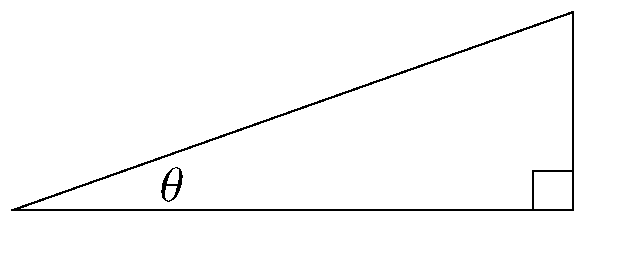
\includegraphics[height=3cm]{trig-substitution/pictures/08-03-ex3a.pdf}%
%}%
%\only<handout:0| 20>{%
%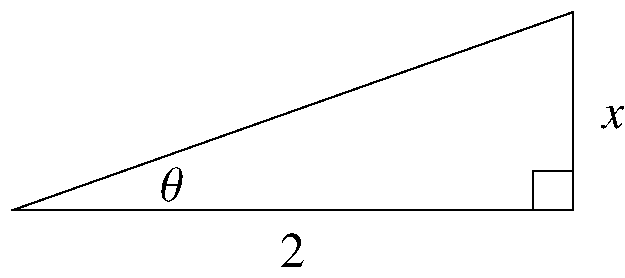
\includegraphics[height=3cm]{trig-substitution/pictures/08-03-ex3b.pdf}%
%}%
%\only<21->{%
%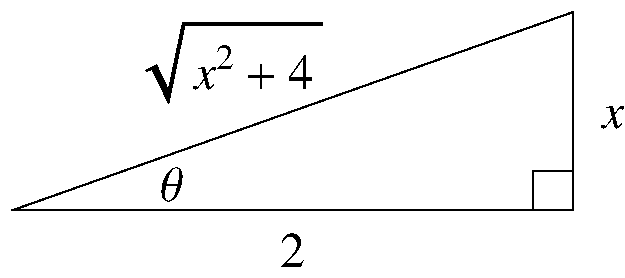
\includegraphics[height=3cm]{trig-substitution/pictures/08-03-ex3c.pdf}%
%}%
\end{center}
\end{columns}
\abovedisplayskip=0pt
\belowdisplayskip=0pt
\uncover<11->{
From the triangle we have 
\[
\frac{\sqrt{x^2+4}}{2} = \uncover<12->{\sec\theta}\uncover<13->{\textrm{ so } \sqrt{x^2+4}=2\sec\theta} 
\]
\abovedisplayskip=0pt
\belowdisplayskip=0pt
\begin{eqnarray*}
\uncover<14->{%
\int \frac{\diff x}{x^2\sqrt{x^2+4}}%
}%
& \uncover<15->{ = } & %
\uncover<15->{%
\int\frac{2\sec^2 \theta \diff \theta}{4\tan^2 \theta \cdot  2\sec \theta}
}%
\uncover<16->{%
 = \frac{1}{4}\int \frac{\cos \theta}{\sin^2\theta} \diff \theta
}\\%
\uncover<17->{%
}%
& \uncover<18->{ = } & %
\uncover<18->{%
\frac{1}{4} \int \csc\theta \cot \theta \diff \theta
}\\%
& \uncover<19->{ = } & %
\uncover<19->{%
 -\frac{\csc \theta}{4} + C
}%
\uncover<20->{%
=  -\frac{\sqrt{x^2+4}}{4x} + C
}%
\end{eqnarray*}
} %
\end{example}
\end{frame}
% end module trig-substitutions-ex3-version-2
